\documentclass{boi2014-de}

\usepackage{enumitem}
\usepackage{todonotes}

\renewcommand{\DayNum}{0}
\renewcommand{\TaskCode}{network}
\renewcommand{\TaskName}{Computer-Netzwerk}

\begin{document}
    Die $N$ Computer im Computerraum einer Schule sind mit Kabeln vernetzt.
    Zwischen je zwei verschiedenen Computern gibt es entweder eine direkte Verbindung per Kabel
    oder eine Verbindung über ``Drittcomputer''.  Nachrichten, die zwischen zwei
    Computern verschickt werden, nehmen immer die kürzeste Route, mit minimal
    vielen Drittcomputern.
        
    Adam und Billy nutzen verschiedene Computer $a$ und $b$ in diesem Raum
    und wollen die kürzeste Route zwischen ihren Computern bestimmen.
    Die Kabelverbindungen kennen sie nicht, aber sie können Nachrichten zwischen
    den Computern verschicken und dabei die Anzahl der Drittcomputer auf der Route
    zwischen den Computern bestimmen.

    Hilf Adam und Billy:

    \Task
    Bestimme die kürzeste Route zwischen Computern $a$ und $b$ mit
    Hilfe einer begrenzten Anzahl von Nachrichten.

    \Implementation
    Implementiere eine Prozedur \method{findRoute(N, a, b)} mit den folgenden Parametern:

    \begin{itemize}
        \item $N$ -- die Anzahl der Computer
            (die Computer sind von $1$ bis $N$ nummeriert)
        \item $a, b$ -- die Nummern von Adams and Billys Computern
            ($a \neq b$ und $1 \le a, b \le N$)
    \end{itemize}

    Deine Prozedur \method{findRoute} kann die Funktion \method{ping(i, j)} aufrufen.
    Deren Parameter sind die Nummern zweier verschiedener Computer
    ($i \neq j$ and $1 \le i, j \le N$).
    Sie liefert die Anzahl der Drittcomputer auf der Route von $i$ nach $j$.

    Deine Prozedur \method{findRoute} muss eine kürzeste Route
    einer Nachricht von $a$ nach $b$ angeben,
    indem sie wiederholt die Prozedur \method{travelTo(k)} aufruft.
    Deren Parameter ist die Nummer des jeweils nächsten Computers auf der Route
    ($1 \le k \le N$). Die Nachricht startet bei $a$, und bei einem Aufruf von
    \method{travelTo(k)} geht sie zu Computer $k$.

    Damit ein Testfall als gelöst gilt, müssen -- zusätzlich zu Laufzeit-
    und Speicherlimits -- folgende Bedingungen eingehalten werden:

    \begin{itemize}
        \item Wenn die Prozedur \method{findRoute} terminiert, muss die Nachricht bei $b$ sein.
        \item Zwei Computer, die auf der Route der Nachricht unmittelbar aufeinander folgen, 
        müssen direkt per Kabel verbunden sein.
        \item Die Nachricht muss eine kürzeste Route nehmen.
        \item Die Anzahl $M$ der Aufrufe von \method{ping} 
        darf eine gegebene Grenze nicht überschreiten (s.~Abschnitt Bewertung).
        \item Die Funktion \method{ping} und die Prozedur \method{travelTo} 
        dürfen nur mit erlaubten Parameterwerten aufgerufen werden.
    \end{itemize}

    \Example
    Schau dir das Beispiel in der Abbildung unten an (Kreise sind Computer, Linien sind Kabel).
    Es gibt $N = 4$ Computer, Adam und Billy nutzen die Computer $a = 1$ und $b = 4$.

    \begin{wrapfigure}[1]{r}{5cm}
        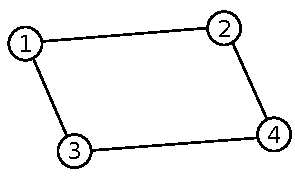
\includegraphics{network-example}
    \end{wrapfigure}

    Nun wird deine Prozedur \method{findRoute} aufgerufen:
    \begin{figure}[H]
        \centering
        \method{findRoute(4, 1, 4)}.
    \end{figure}

    Sie könnte sich z.B. so verhalten:

    \begin{figure}[H]
        \centering
        \method{ping(1, 4)} wird aufgerufen und liefert $1$, \\
        \method{ping(1, 2)} wird aufgerufen und liefert $0$, \\
        \method{ping(2, 4)} wird aufgerufen und liefert $0$.
    \end{figure}

    Diese Information genügt, um die folgende kürzeste Route von $1$ nach $4$ zu bestimmen:
    $1 \to 2 \to 4$.  Diese Route sollte nun so angegeben werden:

    \begin{figure}[H]
        \centering
        \method{travelTo(2)} wird aufgerufen, \\
        \method{travelTo(4)} wird aufgerufen, \\
        \method{findRoute} terminiert.
    \end{figure}

    \Scoring
    In allen Subtasks gilt:  $2 \le N \le 1000$

    \begin{description}

        \item[Subtask 1 (25 Punkte):] zwischen je zwei Computern gibt es genau eine kürzeste Route; 
        $M$ darf nicht größer sein als $2N$.
        \item[Subtask 2 (25 Punkte):] $M$ darf nicht größer sein als $N^2$.
        \item[Subtask 3 (25 Punkte):] $M$ darf nicht größer sein als $4N$.
        \item[Subtask 4 (25 Punkte):] $M$ darf nicht größer sein als $2N$.
    \end{description}

    \Constraints
    \begin{description}
        \item[Time Limit:] 1 s.
        \item[Memory Limit:] 64 MB.
    \end{description}

    \Experimentation
    Der Beispielgrader auf deinem Computer liest vom Standardinput.
    Die erste Eingabezeile sollte vier Integer enthalten: $N, a, b$ und das Limit für $M$ (die Anzahl der ping-Aufrufe).
    Die nächsten $N$ Zeilen sollten je $N$ Integer enthalten, die das Netzwerk beschreiben:
    Die $j$-te Zahl in Zeile $i$ ($i \neq j$) gibt die Anzahl der Drittcomputer auf einer kürzesten Route von $i$ nach $j$ an.
    Die Einträge für $i = j$ werden nicht beachtet.

    Die folgende Eingabe entspricht dem obigen Beispiel, mit einem Limit von 100 für $M$.

    \begin{center}
        \begin{tabular}{p{4cm}}
            {\tt
                4 1 4 100 \newline
                0 0 0 1 \newline
                0 0 1 0 \newline
                0 1 0 0 \newline
                1 0 0 0
            }
        \end{tabular}
    \end{center}

\end{document}

